\chapter{State of the Art} \label{chap:State of the Art}
% introduction

\section{Implementation of Reactive Systems}
	\subsection{Reactive Functional Programming}
	A Reactive Functional Programming (from now on \emph{Reactive Programming}) framework removes a lot of boilerplate code the developer usually has to implement to propagate changes and event throughout a software system. It advances the well known Observer Design Pattern and overcomes several short-comings of that approach. In the Observer Design Pattern, a Subject propagates changes to its state to a list of prior registered Observers. In contrast to an Observable (also called Signal) in Reactive Programming, which can provide multiple values over time as a stream, a Subject can only return one value - its state.
	In addition to Observables which provide varying values over time, a Reactive Programming implementation usually contains a possibility to handle discrete events over time called Events or Event Streams\cite{BaconJS}.
	
	What we refer to as an Observable actually consists of three parts - a Producer that produces values over time, the actual Observable that stores these values, and the Observer that notifies all Subscribers (sometimes also called Consumers). The notification of the Subscribers is specific to \emph{push-based} systems where the values are pushed through the reactive system when a new value arrives, rather than being pulled in a pull-based system on demand if a value is requested by a Subscriber of an Observable or any of its descendants (other Observables that depend upon it).
	Observables can also be categorized as \emph{hot} or \emph{cold} \cite{HotVsCold}. A \emph{cold} Observable will create a new Producer each time a Subscriber subscribes to its Observer. The Producer will be destroyed when the Subscriber unsubscribes - this is referred to as the unicast approach. On the other hand all Subscribers to a \emph{hot} Observable will (usually) share one Producer - this is referred to as the multicast approach.
	
	The declarative functional programming style limits side-effects and is usually implemented with many \emph{pure} functions as operators that can be used to transform, combine or change behavior of Observables and Event Streams. The operators return a new Observable that depends upon the Observable on which the operator was used. Using these operators, the developer declares dependencies between observables, which creates more comprehensible program code and structure \cite[Why Reactive Programming?]{ReactiveInspector} than imperative programming style would produce. 
	

	\subsection{RxJs and BaconJs}
	Although there are many JavaScript implementations of the reactive design pattern like Cycle\cite{CycleJS}, Kefir\cite{KefirJS} or  Most\cite{MostJS}, this section is focused on ReactiveX for JavaScript (RxJS) \cite{RxJs} and Bacon (BaconJS) \cite{BaconJS}, because these are the frameworks/libraries the Chrome Reactive Inspector currently supports. A comprehensible list of reactive frameworks and libraries for JavaScript can be found at \cite{FRPJSList}.
	
	\textbf{Rx.js}\\
	Reactive Extensions for JavaScript or RxJS is the JavaScript implementation of ReactiveX. There are also ReactiveX implementations for many programming languages, for example Java (RxJava), Scala(RxScala) or C\#(Rx.NET). In extension to the basic concepts of Reactive Programming, RxJS implements Subjects and Schedulers. A Subject represents the implementation of an Event Stream and is the only possibility to realize a multicast Observable, since Observables are \emph{cold} Observables in RxJs. They can be Observer and Observable at the same time. To convert a \emph{cold} Observable into a \emph{hot} one the functions \emph{share} or \emph{publish} can be used which will internally use a Subject to track the shared Producer. A Subject will terminate once the last Subscriber unsubscribes. Schedulers are centralized dispatchers that are used to control concurrency that allow to influence the scheduling behavior when asynchronous functions are called e.g. \emph{setTimeout}\cite{RxJsDocu}.
	Observers raise special events if the Observable is completed or reaches an error state - the Observable will not be reusable after wards (even if it is a Subject), which is a main difference to the later discussed BaconJS. RxJs provides many utility functions to convert values, arrays or events into observables \cite{ThesisBaradur}. A basic example of RxJs code to show the general structure can be seen in listing \ref{lst:Rx} (Source: \cite{RxJsDocu} under manual/overview.html).
	The latest stable version of RxJs is version 5.5.6 with version 6.0.0-alpha already under active development. RxJS is licensed under the Apache 2.0 license and the source code is publicly available on GitHub \cite{RxJs}.

	\begin{lstlisting}[language=JavaScript, caption={Example of RxJs code.},label={lst:Rx}]
	var button = document.querySelector('button');
	Rx.Observable.fromEvent(button, 'click')
	.throttleTime(1000)
	.scan(count => count + 1, 0)
	.subscribe(count => console.log(`Clicked ${count} times`));
	\end{lstlisting}
	
	\textbf{Bacon.js}\\
	The basic concepts of BaconJS \cite{BaconJS} are Properties - which represent the Observables - and EventStreams that handle distinct events. 
	In contrast to RxJS, BaconJS'S Properties are always \emph{hot} Observables. In addition an Error in a EventStream or Property will not cause it to terminate. Errors are therefore handled as any other value which provides more fine grained control for the developer. However, the \emph{endOnError} function can be used if the termination is desired. 
	Another advantage of BaconJs is the \emph{spy} function, which can be used to observe the internal workings and greatly reduces the required effort to create complementary tooling like CRI or RxFiddle. It can also be used to easily create extensive logging without modifying the rest of the reactive application source code. According to the author(s), BaconJS was started because they got frustrated with RxJs, because its source code was not publicly available at the time and the documentations was minimal. They also claim that BaconJS has a more consistent and glitch free stream/property behavior \cite{BaconJSRepo}, but they also explain that RxJs has less overhead and therefore a better performance. 
		\begin{lstlisting}[language=JavaScript, caption={Example of Bacon.js code.},label={lst:Bacon}]
	$("#username input").asEventStream("keyup")
	.map(function(event) {
	return $(event.target).val();
	})
	.toProperty("")
	\end{lstlisting}
	The latest stable version of BaconJS is version 2.0.0 and it is still under active development. BaconJS is licensed under the MIT license and the source code is publicly available on GitHub \cite{BaconJSRepo}.

	While BaconJS is a newer Reactive Programming library and was developed to handle some short-comings of RxJS, according to the GitHub statistics RxJS has still a much larger community. RxJs has 387 watches, 10540 stars, 991 forks and 185 contributors for the currently active repository and BaconJS has 156 watches, 5839 stars, 328 forks and 83 contributors in total (last accessed: 31.1.2018 18:22).
	In addition, since RxJS started earlier and due to its similarity to other ReactiveX implementations in other languages, there exist a multitude of tools and utility libraries that are exclusive for RxJS - including RxFiddle.

\subsection{Debugging Reactive Code}
The violation of a syntax rule of in a programming language such as missing control characters, misspelled keywords etc. are syntax errors and can be detected by most IDEs very precisely, but logical errors are harder to track down. Modern IDEs use breakpoints including conditional breakpoints, step by step execution, event logging, stack traces and many more. Due to reactive programming being declarative, breakpoints, the most useful feature for in-depth code and state inspection at a precise point during the applications execution can not be used as easily. For some IDE even chained function call provide a obstacle because there breakpoints are line and not character position based. But even if the IDE can handle breakpoints inside lambda functions for the usual navigation features like \emph{Step Over} and \emph{Step Into} it is not trivial to balance between providing the necessary fine grained stepping and having to many steps for the developer to iterate. For example one of the most advanced IDEs there is, Visual Studio (2017) for .NET, will step over the whole batch of chained functions if the developer uses \emph{Step Over}, but will step into the first lambda function in the chain if the developer uses \emph{Step Into}. The developer can then use \emph{Step Over} to enumerate the lambda functions passed to the chained functions (see listing \ref{lst:CSharp_LINQ}). This is a very specialized and desirable behavior that will match the intend of the developer most times when using the .Net Framework built in \emph{.NET Language-Integrated Query Expressions} (LINQ), but this behavior will break as soon as a custom function is added to the chain (\emph{DoCustom} in the code example). Now the \emph{Step Into} on line 1 will step into \emph{DoCustom} for each entry in the list and will then step out of the batch of chained functions to line 10. If a similar code example in Bacon.js is debugged with the step-by-step debugging feature of Google Chrome, it will actually step through the Bacon.js library code even if the developer just uses \emph{Step Over}. Because Bacon.js or other reactive programming frameworks are not part of native JavaScript Google Chrome as no means to determine if the user wants to step through the framework code or not.
This example shows that debugging declarative code is still a hard task for modern IDEs, especially if Out-of-Order execution (LINQ Expressions are executed Out-of-Order) is added.
The developers intention is not easy to interpret by the IDE, because there is a multitude of possible steps to take there. The developer could want to debug the custom chained function, they could want to iterate the lambda functions passed as arguments to the chained functions, they could also want to step through the framework functions (Select, Where, OrderBy, etc. which is possible if framework debugging is enabled in Visual Studio 2017 for .NET). 
For big collections, or in the case of reactive programming, observables with many submitted values this problem is also increased by having too many single executions of a lambda function for the developer to step through. Another example for this would be a breakpoint inside a lambda function that is passed to a declarative function (like\emph{Where} in C\# or \emph{map} in Bacon.js) which would halt the application for each element in the collection or data stream.

%TODO: language is c# but the compilation would not complete with "[Sharp]C" as language.
\begin{lstlisting}[language=JavaScript, caption={Simple example of .NET LINQ in C\# to show the steps the visual stidio 2017 for .NET debugger takes while debuggin step-by-step.},label={lst:CSharp_LINQ}]
 var lst = new List<string>{"test1","test2"};
 var result = lst.Select(s => s.ToUpper())
 .Where(s =>
 {
	var b = s.StartsWith("t");
	return !b && s.StartsWith("T");
 })
.OrderBy(s => s)
.DoCustom()
.ToList();
\end{lstlisting}


This shows that a traditional debugger is not suitable to use with declarative programming especially reactive programming. While the the Visual Studio debugger is still somewhat useful to debug LINQ in .Net, because multiple specialized behaviors have been implemented over the years and LINQ expressions will most likely not cover the entire application and are often used to execute short tasks inside an imperative program flow, observables in a reactive application are usually much more intertwined and make up the general flow of the program; making a traditional debugger more of an obstacle.

As described in \cite{MSDN_DebugginObservables} reverting to the most basic debugging technique sometimes called \emph{printf-debugging} (or in the Rx.js terms \emph{do-debugging}), to generate debug outputs or traces by directly modifying the source code, generally provides better results than using advanced features of a traditional debugger.
Some of the shortcomings of this basic technique can be mitigated by using sophisticated tools like shown in \cite{ShinyGraphFromLog} in the section "The Reactive Log" where the log of an application is visualized in a dependency graph containing code pieces as nodes, do-debugging still requires the source code to be modified and polluted with statements that do not contribute to the program logic itself.
% requires manual modification of source code to trace program execution.

%- "lack of abstractions" and "mismatch in the mental model" [paper guido1]. "Traditional debuggers are mostly based on runtime stack information and do not consider any other abstraction within the running code." [Abbas]
% - "Missing dependencies are hard to detect with traditional debuggers." [paper guido1 4.1]

The programming language JavaScript (JS) is, unlike compiled languages, harder to debug, because it is an interpreted script language and the JS code is not compiled before execution. The general advantage of being able to change the code during execution and having no compile time, are shadowed by the fact that many bugs can only be found at runtime. 

%...

Currently there are few tools to help the developer debug reactive applications and apart from RxFiddle (described in detail in section \ref{sec:RxFiddle}) non of them, as far as we known, support debugging reactive JavaScript applications. One of those tools is \cite{ShinyGraphFromLog} as mentioned above. Another is the Reactive Inspector for the Scala language \cite{ReactiveInspector} started and maintained by Prof. Dr. Guido Salvaneschi working in the Software Technology Group of the Technical University of Darmstadt, Germany.
The Reactive Inspector is an extension of the Scala IDE for Eclipse. Many features and the basic concepts taht are implemented in the \emph{Chrome Reactive Inspector(CRI)} originate from the Reactive Inspector; including the representation of observables and their dependencies in a dependency graph called \emph{Reactive Tree}, the possibility to query the history of said %TODO can "said" be used?
 graph or the possibility to search for a specific node in the current graph. They are described in details in section \ref{sec:PreviousCRI}. One main feature of the Reactive Inspector, called \emph{Tree Outline} where the user can quickly jump to different areas of the dependency graph, which is useful for applications with large graphs, is currently not implemented for the CRI.

\section{Previous and Related Work}
In this section we will cover the previous work on the Chrome Reactive Inspector (CRI) as well as RxFiddle which is the main competitor for the CRI because both have a similar goal to help developers debug Reactive Systems in JavaScript with abstract concepts that go beyond traditional debugging.

%TODO: framework vs library - write at the beginning that framework and library may be used interchangeable for convenience.
	\subsection{The Chrome Reactive Inspector}
	\label{sec:PreviousCRI}
	The Chrome Reactive Inspector is based on the Reactive Inspector for Scala \cite{ReactiveInspector} and was developed by the Software Technology Group at the TU-Darmstadt Germany supervised by Prof. Dr. Guido Salvaneshi. It is implemented as a Google Chrome(Chrome) extension that extends the Chrome Developer Tools (DevTools) with another panel that inspects and instruments a target Reactive web application that is using RxJS or BaconJS. Prior to this thesis there have already been two Master theses targeting the CRI that provide the base theory and source code of this thesis.
	%TODO: thesis capatalized?
	\subsubsection{Master Thesis by Waqas Abbas}
	\cite{ThesisAbbas} The main goal of the Master Thesis by Waqas Abbas was to develop and implement a concept for a Chrome extension based on the Reactive Inspector to debug Reactive web applications in JavaScript.
	%TODO: The main - twice
	%TODO: many "to"s
	The main difficulties were to find a viable solution to intercept calls to the reactive frameworks in order to retrieve the necessary information about observables and their dependencies to build a Dependency Graph (called Dependency Tree in \cite{ReactiveInspector}) as well as to gather additional details like variable name that directly correspond to observables and providing them with context by instrumenting the source code. An in-browser solution taken from a demo page \cite{JalangiDemo} of Jalangi was used to instrument and analyze the source code directly. The main Jalangi framework \cite{Jalangi} is currently not usable solely within a browser.
	Abbas also implemented several features to help the developer navigate and examine the Dependency Graph and its history. In this first version of the CRI, the user could already submit History Queries that search the History of the Graph for specific nodes or events like node creation, update or the creation of a dependency. In addition the user could add Reactive Breakpoints - breakpoints that pause the program execution when a specific event occurs - or search for a node in a large Dependency Graph.
	At the time the CRI supported BaconJS\cite{BaconJS} and parts of RxJS\cite{RxJS}. Abbas also added a first batch of small web applications that could be used as test applications to manually verify features of CRI.
		
	\subsubsection{Master Thesis by Pradeep Baradur}
	The main goal of the Master Thesis by Pradeep Baradur was to add full support for RxJS to CRI.
		% main focus of the thesis:
			% support for all RxJS operations and RxJS Subjects -> hard to implement, because there is no uniform way like the Bacon.spy method. For details on the general approach see \cite{ThesisBaradur}. For source code see "rx-interception.js"
		% new features introduced:
			% - support for all operations and Subjects in RxJs
			% - loading of some CRI content scripts only when the CRI panel is opened. Istrumentation only when CRI panel is opened.
			% - find dependencys, dependents
			% - added many test applications
			% - improved reliability
			% - less focus on maintainability but move the project further to being usable in a production environment by adding framework feature support.
			% - rearranged UI, changed many styles to defaullt jquery-ui layout.
		
		\subsubsection{Merging previous efforts}
		
		% The Thesis by Waqas Abbas focused on new implementation and prototypes of features and less on maintainability and reliability.
		
		%- took chrome-reactive-inspector 2 as base and merge all later developed features into it, piece by piece. manually copied changes by Pradeep from Waqas's repository. Hard to detect, changed to match other variable names before committing.
		% - uncompatible git histories - solvable but not much use since the files had separated so much in text character changes, though not so much in logic -> renames and splitting of files
		% - access to many global variables made tracking down dependencies of components hard with mixed contexts - some files with the window object corresponding to contentscripts in the same directory as files with a window object corresponding to the extensions window.
		%TODO: change tone to always present problems as general difficulties instead of shortcomings
		% - merged additional features of Abbas with framework support from Pradeep
		
		\subsubsection{"Special Curicumstances"}
		% demo version of jalangi
		% instrumenting files via scanning the html for script tags
		% -> will not work for module loaders like require.js or ecma6
		% -> will not work with bundled JavaScript code - but since in development there should be a non bundled version available not 
		% a big problem in JavaScript. But for TypeScript since the extension does not support it and when compiling there may already be bundling in place. (#add some text from future here#)
		
		% Shared context through "new Function" that breaks the separation enforced by chrome. To increase consistency and prevent different execution contexts the previous eval was replaced with "new Function" but this does not reduce the security risk.There are other options to execute scripts from a chrome extension but since some of the extension scripts need to share the Rx or Bacon object with the inspected pages JavaScript files there is no other way. ofcorse that breaks the normal isloated world and intodruces a new set of problems like conflicting names. The security risk involved in executing a foreign script in a "trusted" extension context could be reduced if a sandbox was used as described in https://developer.chrome.com/extensions/sandboxingEval. Then all the inspected pages content scripts and some special recording scripts could be executed in that sandbox and transmitt the recorded nodes back via message passing.
		% - Dangers of using eval -> execution in current context. if called from other function, "this" might change. Function() for global with window passed to execute in original context.
		%- Note that  files that are not selected for instrumentation will still generate nodes in the graph, because the Rx and Bacon frameworks will still record interactions, just the information provided by instrumentation is missing.
		%- The Bacon and Rx scripts are prevented from loading so the extensions own files can be used. This is accomplished by filtering all referenced js files in the inspected page for any Bacon or Rx library files and excluding them from the loading process. They need to match version exactly though. This is necessary to guarantee that both work with the same Rx/Bacon object.
	

	\subsection{RxFiddle}
	\label{sec:RxFiddle}
	
	% RxFiddle is the main competitor with CRI since it is the only other tool (that we are aware of) that tackels debugging for reactive JavaScript systems. Currently the only reactive framework that is supported is RxJs.
	% features of RxFiddle
	% limitations: 'one of the limitations of RxFiddle is ... which we tackeld in this work.
		% - requires more setup to use with web sites that have DOM logic and applications with more than one JavaScript files, although it is possible according to the author \cite{RxFiddleTutorials}.
		% - the variable names in the source code are not displayed in the ui. RxFiddle instruments RxJs to collect its data, not the source code itself like CRI.
		% - fast updating observables like "interval" since each value update creates a new marble for the observable, the view becomes encoumbered fast with this type of observables. As of this moment CRI also generates one or more steps for each update (if the node is not explicitly excluded), but it is easier to examine the value of a node in the first or last few steps (jump to the step and use the next/previous button). CRI can also query the result which provide means to cope with large dependency graphs or histories. In RxFiddle the limitating factor for the fine grained stepping is the available space and resulting overplotting of the value-marbles since the examination is implemented via tooltips on mouseover. For performance comparison see \ref{sec:PerformanceEvaluation}.
		
		% - like the author explained in "https://github.com/hermanbanken/RxFiddle/issues/6" the web app can not work with large applications properly. The displaying of large applications in one graph is hard for both tools \ref{sec:RapidlyUpdatedObservables}, but RxFiddle needs more spaces for a single reactive operator than CRI. A large dependency graph with descriptive nodes is easier to examine than a large marble diagram that only shows information on nodes in tooltips except in the details view of a currently selected node so finding the desired node/operation is not as easy. RxFiddle also has performacne issue while rendering huge diagrams according to the author. RxFiddle would porbably need another view to appropiately cope with such large applications to help the user navigate and give an overview, although for mid-sized applications the graph on the left side where a user can choose which operation to examine can serve this purpose - As mentioned earlier RxFiddle does not porvide variable names which may lead to confusion of nodes if similar observables are in the same application.
		% As of now, CRI does not support multiple variables having the same name. The author describes some other options like priority ranking in the GitHub issues for the RxFiddle repository \cite[Issues]{RxFiddleGitHub}.
		% - as mentioned erlier RxFiddle onyl supports RxJs while CRI also supports Bacon.js
	% - The author plans to support multiple collectors in the future for web applications, RxScala, RxJava, RxSwift and/or RxNet (source: "https://rxfiddle.net/tutorials.html#attached") which would provide the necessary data collection on one of these platforms and transmit this data to the RxFiddle tool/web-application to be able to use the same debugging environment (RxFiddle) with any of these platforms.



% end of state of the art chapter
%----------------------------------------------------------------------------
%latex sample code:



%\begin{figure}[!h]
%	\centering
%	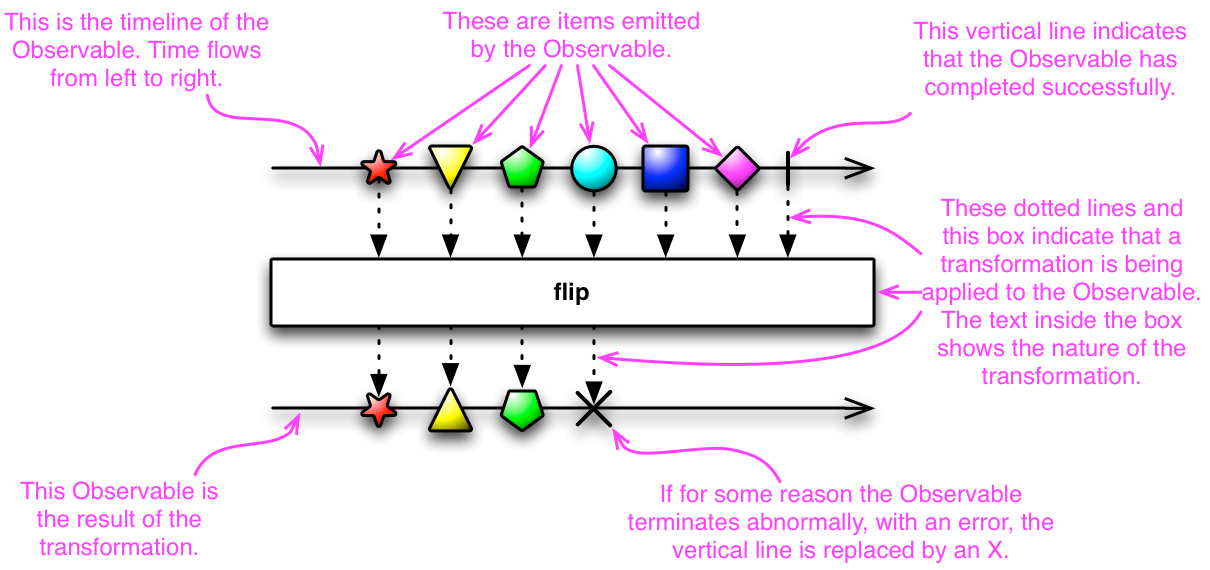
\includegraphics[scale=0.5,trim=0 0 0 0]{gfx/rxjs-reactive-pattern2.png}
%	\caption{Reactive pattern \protect\cite{ReactiveXobservable}}
%	\label{fig:rxjs-reactive-pattern}
%\end{figure}

\textbf{Observable and Observer}\\
Placeholder

\textbf{Operators}
\label{subsec:Operators}\\

\textbf{RxJS Code Structure}\\
Placeholder
\begin{lstlisting}[language=JavaScript, caption=RxJS Simple Example, label={lst:RxJS_Simple_Example}]
// 1. Srouce Observable Creation
var sourceObservable = Rx.Observable.interval(1000);
// 2. Transformation by applying different operators
var transformedObservable = sourceObservable.map(function(x) {
		return x * 10;
	})
	.filter(function(x) {
		return x !== 20
	})
// OUTPUT
Next: 0
Next: 10
Next: 30
Next: 40
Next: 50
Completed
\end{lstlisting}

\subsection{Bacon.js}

\textbf{EventStream and Property}\\
Placeholder

